\documentclass[12pt]{beamer}
%\documentclass[handout]{beamer}
%\usepackage{pgfpages}
%\mode<handout>{\setbeamercolor{background canvas}{bg=black!20}}
%\pgfpagesuselayout{2 on 1}[letterpaper,border shrink=5mm]
\usepackage{CJKutf8} 
\usepackage{graphics,soul,xcolor,color}
\usepackage{hyperref}
\usepackage{pythonhighlight}
\usepackage[normalem]{ulem} % use normalem to protect \emph
%\mode<presentation>{\usetheme{Warsaw}}
\usetheme{Boadilla}
%\usetheme{CambridgeUS}
%\usetheme{Warsaw}
\usecolortheme{dolphin}
\usepackage{tikz}
\usetikzlibrary{mindmap}
\title[Reverse Engineering Algorithmic Mechanism Behind WeChat Red Envelope]{Reverse Engineering Algorithmic Mechanism Behind WeChat Red Envelope}
\author{Qifan Zhang}
\institute[ShanghaiTech]{47422183\\zhangqf@shanghaitech.edu.cn\\School of Information Science and Technology\\ShanghaiTech University}
\date{January 19, 2018}
\begin{document}

\begin{frame}
    \titlepage
\end{frame}

\begin{frame}
  \frametitle{Outline}
  \tableofcontents
\end{frame}

\AtBeginSection[]
{
\begin{frame}{Outline} \tableofcontents[currentsection]
    \end{frame}
}




\section{Introduction}
\begin{frame}{Introduction}
	\begin{itemize}
		\item 10 \emph{yuan} for 5 people each time, 80 trials as prior distribution
		\item guess and build model over prior distribution
		\item test my model by 100 posterior trials
		\item All cell phones used in our experiments are conducted on \emph{WeChat} 6.6.1 on \emph{iOS}.
	\end{itemize}
\end{frame}

\section{Model and Algorithms}
\begin{frame}{Prior Distribution}
	\begin{itemize}
		\item the first participant \textbf{will never get more than \(\frac{2}{5}\) of the total money (i.e. 4 \emph{yuan})}
		\item \textbf{define money gotten by the \(j\)th participant is \(X_j\)}
	\end{itemize}
\end{frame}

\begin{frame}{Prior Distribution of \(X_1\)}
	\begin{figure}[!ht]
		\centering
		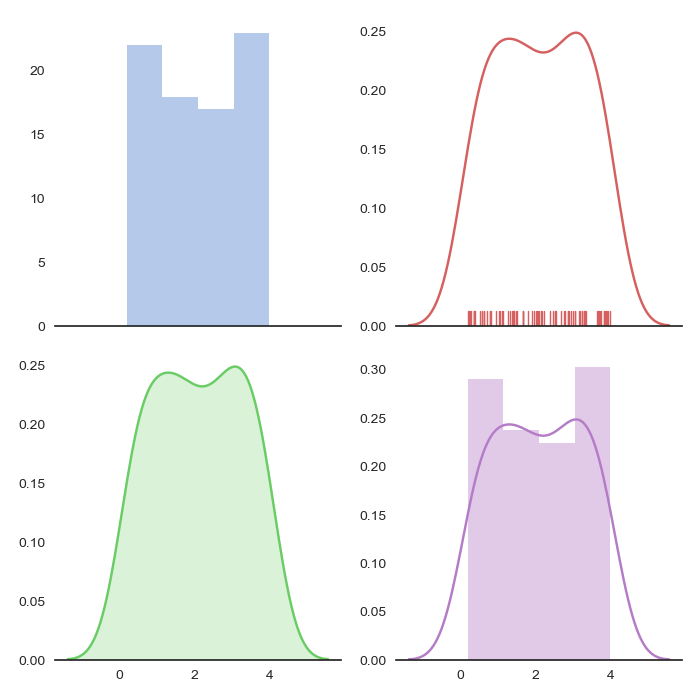
\includegraphics[width=0.5\columnwidth,height=0.5\linewidth]{fig/10_1.png}
	\end{figure}
\end{frame}	

\begin{frame}{Prior Distribution of \(X_2\)}
	\begin{figure}[!ht]
		\centering
		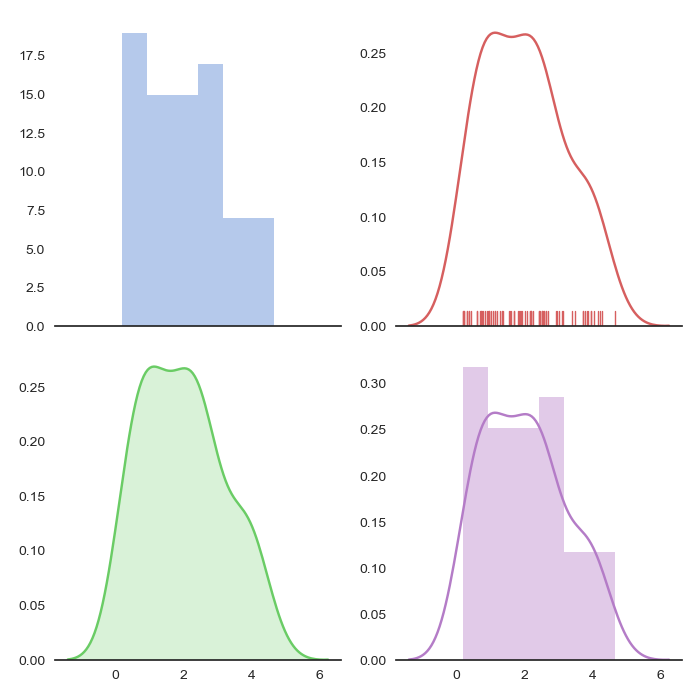
\includegraphics[width=0.5\columnwidth,height=0.5\linewidth]{fig/10_2.png}
	\end{figure}
\end{frame}	

\begin{frame}{Prior Distribution of \(X_3\)}
	\begin{figure}[!ht]
		\centering
		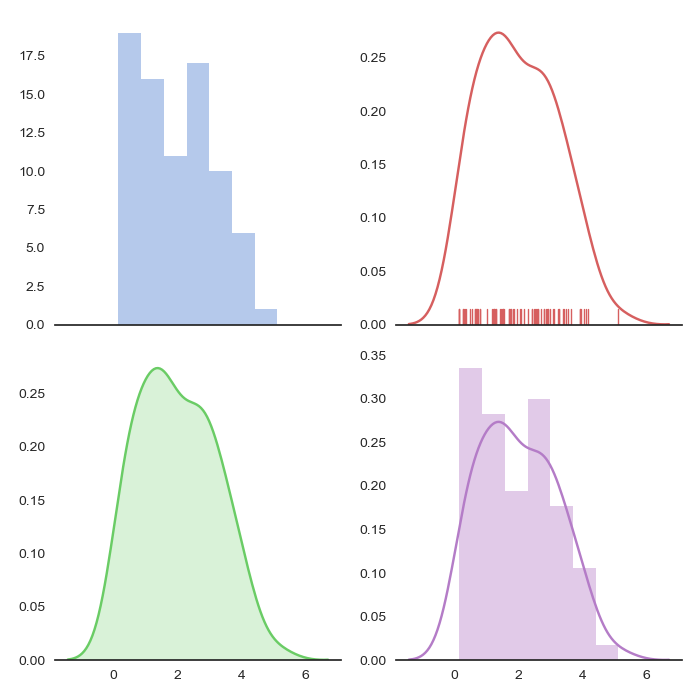
\includegraphics[width=0.5\columnwidth,height=0.5\linewidth]{fig/10_3.png}
	\end{figure}
\end{frame}

\begin{frame}{Prior Distribution of \(X_4\)}
	\begin{figure}[!ht]
		\centering
		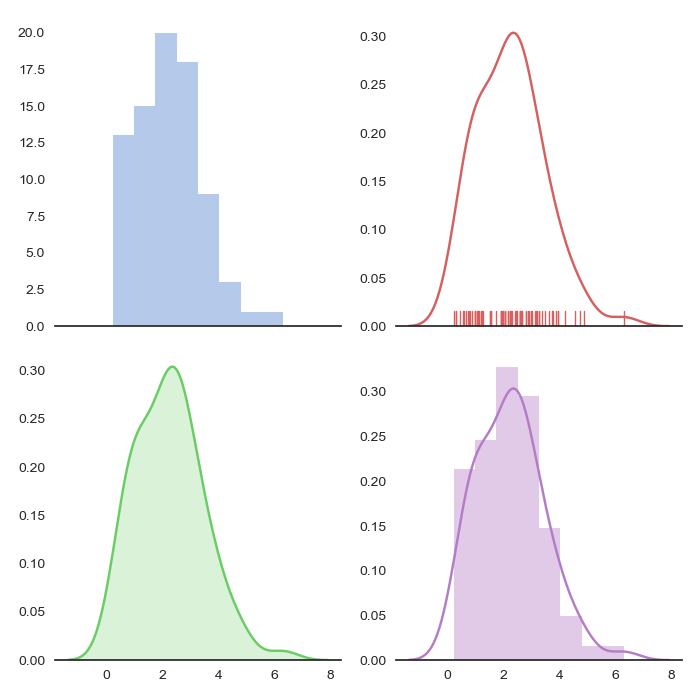
\includegraphics[width=0.5\columnwidth,height=0.5\linewidth]{fig/10_4.png}
	\end{figure}
\end{frame}

\begin{frame}{Prior Distribution of \(X_5\)}
	\begin{figure}[!ht]
		\centering
		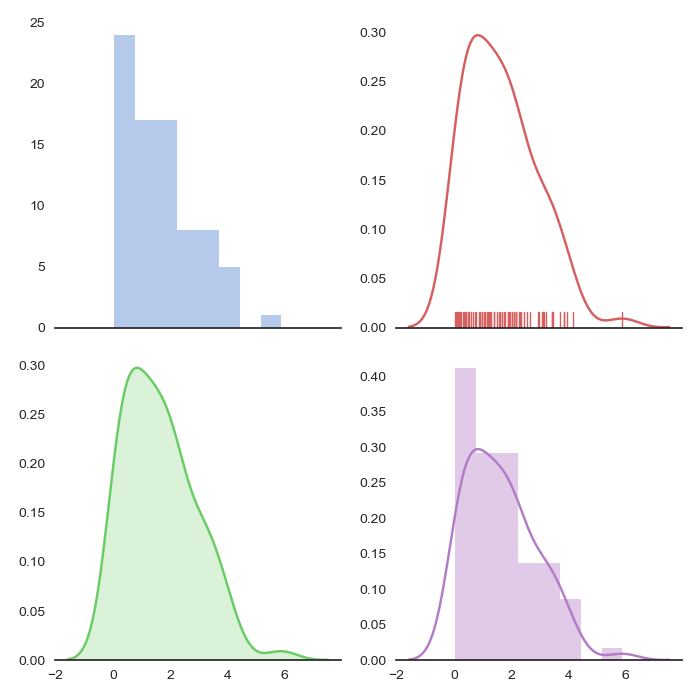
\includegraphics[width=0.5\columnwidth,height=0.5\linewidth]{fig/10_5.png}
	\end{figure}
\end{frame}	

\begin{frame}{Overall Prior Distribution}
	\begin{figure}[!ht]
		\centering
		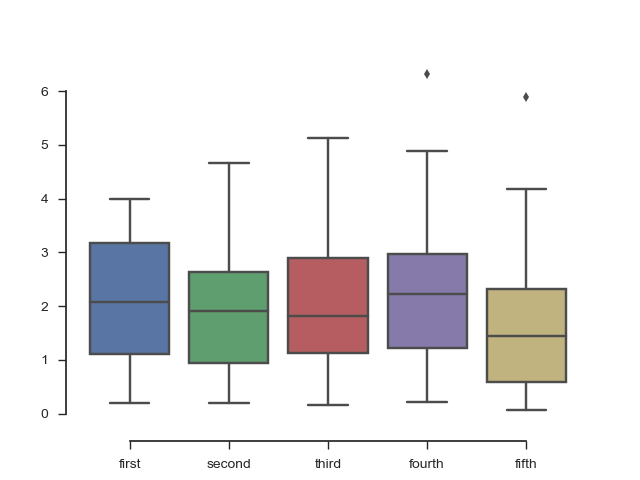
\includegraphics[width=0.5\columnwidth,height=0.5\linewidth]{fig/10_Overall.png}
	\end{figure}
\end{frame}

\begin{frame}{Intuitive Results from Prior Distribution}
	\begin{itemize}
		\item no red envelop for the \emph{first} participant is larger than \emph{yuan}
		\item for the \emph{first} participant, the amount of money distributes nearly uniformly from 0 to 4
		\item I also found that in a 100-\emph{yuan} red envelop, the first participant could get at most 40 \emph{yuan} and in a 1-\emph{yuan} red envelop, the first participant could get at most 0.4 \emph{yuan}.
	\end{itemize}
\end{frame}

\begin{frame}{Distribution for \(X_1\)}
	From \emph{Intuitive Results from Prior Distribution}, I guess that in a 10-\emph{yuan} red envelope for 5 participants:
	\begin{displaymath}
		X_1\sim Unif(0,4)
	\end{displaymath}
\end{frame}

\begin{frame}{Distribution for \(X_2,X_3,...,X_5\)}
	Inspired from \(X_1\):
	\begin{itemize}
		\item do \(X_2,X_3,...,X_5\)\ follow \emph{Uniform Distribution}?
		\item if so, what is distribution domain for each of them?
	\end{itemize}
\end{frame}

\begin{frame}{Distribution for \(X_2,X_3,...,X_5\)}
	After several times of guessing, trying, verifying and correcting, I found a perfect model:
	\[
		\begin{split}
			X_j|X_1,X_2,...,X_{j-1}&\sim Unif(0,\frac{2(n-\sum_{i=1}^{4}X_i)}{5-j})\ \ 2\leq j\leq 4
			\\
			X_5&=n-\sum_{i=1}^{4}X_i
		\end{split}
	\]
\end{frame}

\begin{frame}{Generalized Distribution for \(X_1,X_2,...,X_n\)}
	Then I generalize the model fora \(n\)-\emph{yuan} red envelop for \(m\)\ participators:
	\[
		\begin{split}
			X_1&\sim Unif(0,\frac{2n}{m})
			\\
			X_j|X_1,X_2,...,X_{j-1}&\sim Unif(0,\frac{2(n-\sum_{i=1}^{j-1}X_i)}{m+1-j})
			\\
			&2\leq j\leq m-1
			\\
			X_m&=n-\sum_{i=1}^{m}X_i
		\end{split}
	\]	
\end{frame}

\section{Simulation Results}
\begin{frame}{Stimulation Code}
	I use \emph{Python} programming language to stimulate the process of giving out red envelopes based on my model and algorithm.
\end{frame}

\begin{frame}{Stimulation Code}
\inputpython{Stimulation.py}{1}{18}
\end{frame}

\begin{frame}{Stimulation Results}
	I generate 100 cases for a 10-\emph{yuan} red envelop for 5 participators. Results are below:
\end{frame}

\begin{frame}{Stimulation Result for \(X_1\)}
	\begin{figure}[!ht]
		\centering
		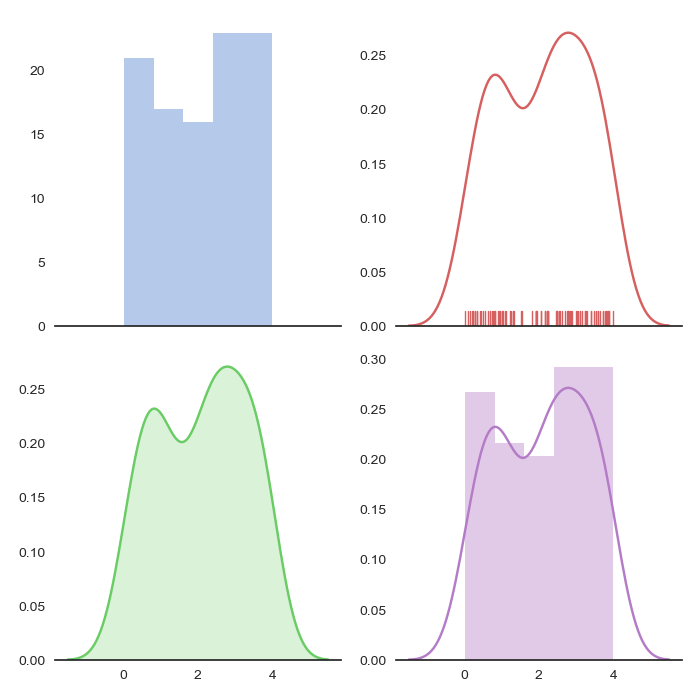
\includegraphics[width=0.7\columnwidth,height=0.6\linewidth]{fig/output_1.png}
	\end{figure}
\end{frame}

\begin{frame}{Stimulation Result for \(X_2\)}
	\begin{figure}[!ht]
		\centering
		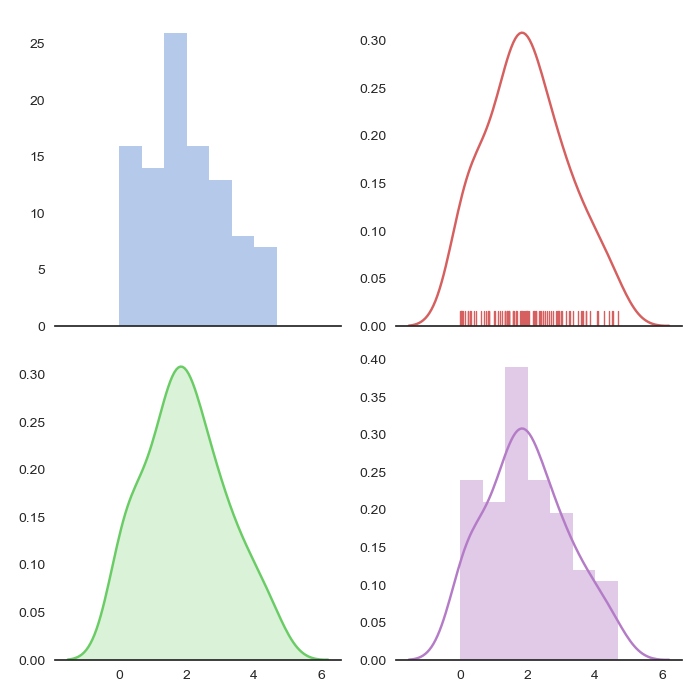
\includegraphics[width=0.7\columnwidth,height=0.6\linewidth]{fig/output_2.png}
	\end{figure}
\end{frame}

\begin{frame}{Stimulation Result for \(X_3\)}
	\begin{figure}[!ht]
		\centering
		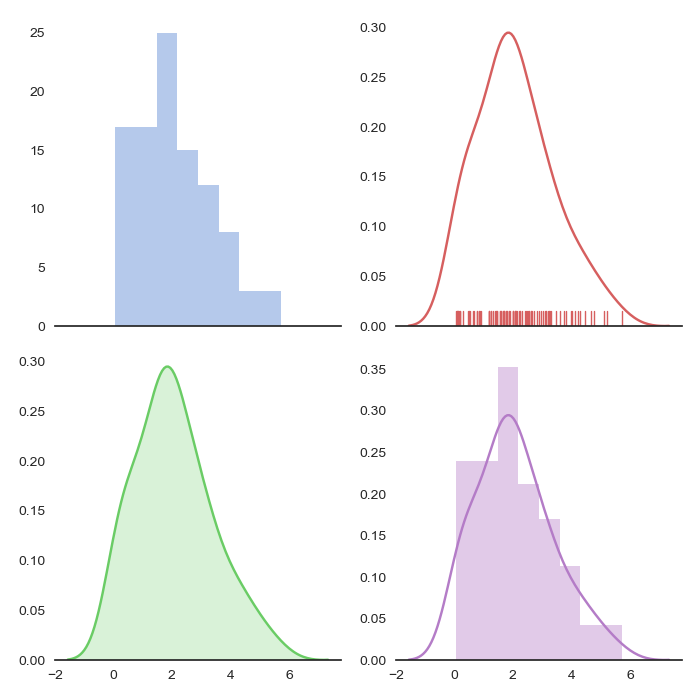
\includegraphics[width=0.7\columnwidth,height=0.6\linewidth]{fig/output_3.png}
	\end{figure}
\end{frame}

\begin{frame}{Stimulation Result for \(X_4\)}
	\begin{figure}[!ht]
		\centering
		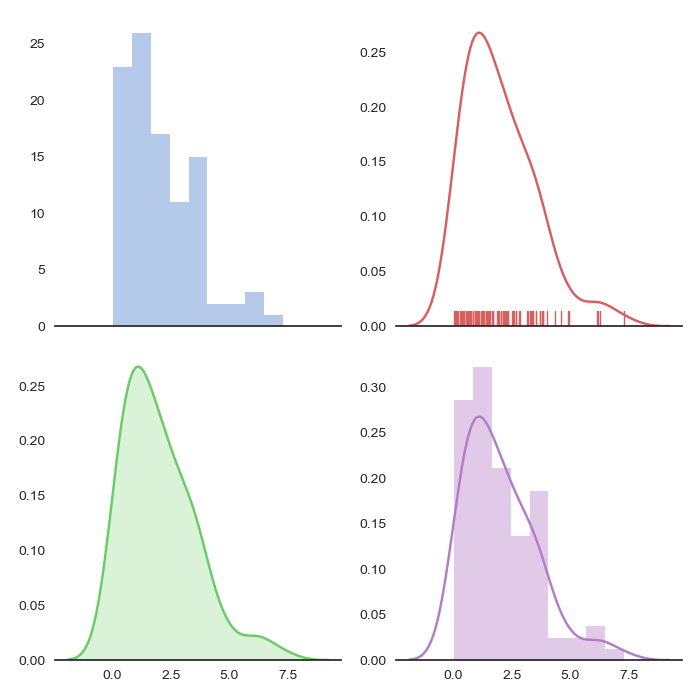
\includegraphics[width=0.7\columnwidth,height=0.6\linewidth]{fig/output_4.png}
	\end{figure}
\end{frame}

\begin{frame}{Stimulation Result for \(X_5\)}
	\begin{figure}[!ht]
		\centering
		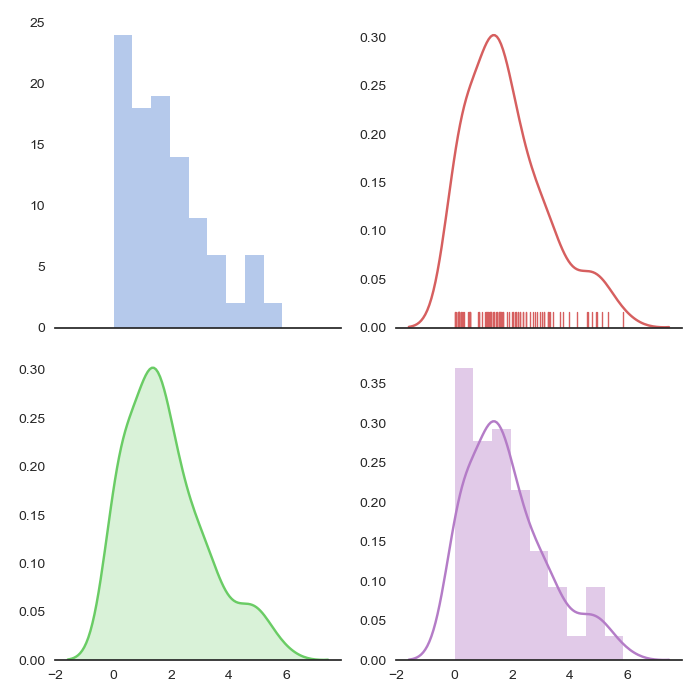
\includegraphics[width=0.7\columnwidth,height=0.6\linewidth]{fig/output_5.png}
	\end{figure}
\end{frame}

\begin{frame}{Overall Stimulation Distribution}
	\begin{figure}[!ht]
		\centering
		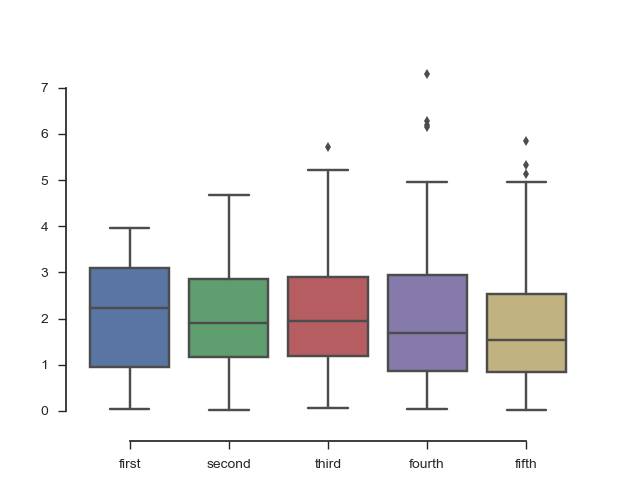
\includegraphics[width=0.7\columnwidth,height=0.6\linewidth]{fig/output.png}
	\end{figure}
\end{frame}

\begin{frame}{Stimulation Conclusion}
	Intuitively, my model satisfies real trials very well.
	\\
	In detail:
	\begin{itemize}
		\item every participant has a similarly-same mean of money.
		\item money of latter participants' red envelopes has \textbf{larger variance} than former participants'.
	\end{itemize}
\end{frame}

\begin{frame}{Enhanced Stimulation}
	To prove my intuitive insights:
	\begin{itemize}
		\item \textbf{Assuming that my model is correct}, we could only do a large number of trials to gain a nearly perfect mean and variance.
		\item I do 1 million times of trials and get the result.
	\end{itemize}
\end{frame}


\begin{frame}{Enhanced Stimulation Result}
	\begin{figure}
		\centering
		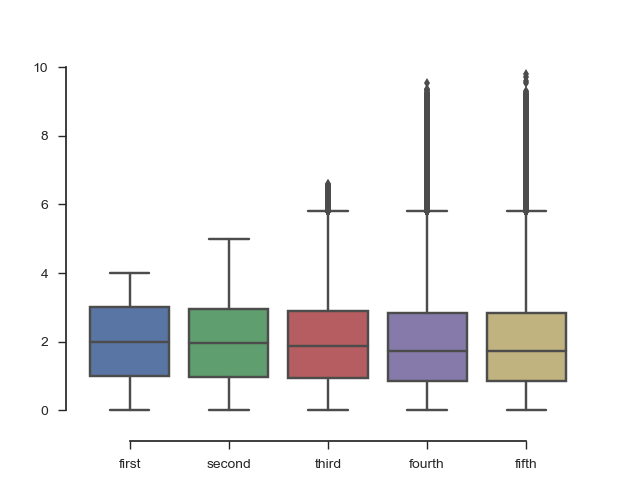
\includegraphics[width=0.7\columnwidth,height=0.6\linewidth]{fig/Stimulation.png}
	\end{figure}
\end{frame}

\begin{frame}{Enhanced Stimulation Conclusion}
	\begin{itemize}
		\item Mean of the amount of money is \textbf{really the same} (\(\approx2\))
		\item Variance is getting larger with rank of the participant getting larger.
	\end{itemize}
	The second proved insight explains why we feel the distribution of the \emph{third, fourth and fifth} participants' amount of money \emph{not perfectly} accord with our stimulation results.
\end{frame}

\section{Conclusion}

\begin{frame}{Conclusion- \emph{from Academic Side}}
	Define \(X_j\)\ as the money the \(j\)th participant gets for a \(n\)-\emph{yuan} red envelop for \(m\)\ participators.
	\\
	The distribution is:
	\[
		\begin{split}
			X_1&\sim Unif(0,\frac{2n}{m})
			\\
			X_j|X_1,X_2,...,X_{j-1}&\sim Unif(0,\frac{2(n-\sum_{i=1}^{j-1}X_i)}{m+1-j}
			\\
			&2\leq j\leq m-1
			\\
			X_m&=n-\sum_{i=1}^{m}X_i
		\end{split}
	\] 
\end{frame}

\begin{frame}{Conclusion- \emph{from Academic Side}}
	\begin{itemize}
		\item Mean of the amount of money is \textbf{really the same}.
		\item Variance is getting larger with rank of the participant getting larger.
	\end{itemize}
\end{frame}

\begin{frame}{Conclusion- \emph{from Intuition Side}}
	\begin{itemize}
		\item The faster you participate in the \emph{Red Envelope} game, the more stable the expected amount of money you get is
		\item If you want to try your luck and get larger amount of money, please participate in this game a little later.
	\end{itemize}
	Of course, it is only meaningful when you \textbf{have grabbed} a red envelope.
\end{frame}

\section{Acknowledgment}

\begin{frame}{Acknowledgment}
	During this project, I collaborated and discussed with my classmates \textbf{Cheng'an Wang}, \textbf{Huifan Zhang}, and \textbf{Letong Wang}.
	\\
	Data of real trials are collected by \textbf{Cheng'an Wang}, \textbf{Huifan Zhang} and me.
	\\
	I got inspiration of \emph{Uniform Distribution} from \emph{Zhihu}\(\left[ 1 \right]\) and \emph{Zybuluo.com}\(\left[ 2 \right]\). I think the idea \emph{Uniform Distribution} is quite excellent, but the author does not choose a right domain for it.
	\\
	All the resources of this report have been pushed to \emph{my Github}\(\left[ 3 \right]\).
\end{frame}

\section{Reference}

\begin{frame}{Reference}
	\begin{itemize}
		\item \(\left[ 1\right]\) https://www.zhihu.com/question/22625187/answer/85530416
		\item \(\left[ 2\right]\) "Brief Introduction to Framework Design of WeChat Red Envelope" https://www.zybuluo.com/yulin718/note/93148
		\item \(\left[ 3\right]\) https://github.com/KevinZhang199803/SI140\_Final\_Project
	\end{itemize}
\end{frame}
\end{document}
